\section{requirement specification}
\label{req_spec}

\subsection{Overview}
\label{overview}

\begin{itemize}
 \item provide status information to MAC
 \item switch radiostate (RX, TX, SLEEP)
 \item send packets to air/channel
 \item receive packets / listen for packets
 \item provide hooks for statistical information
 \item configurable settings
\end{itemize}

\subsection{provide status information to MAC}
\label{stateInfo}

In addition to received packets the physical layer has to provide some other information to the MAC layer.
Some of this information has to be provided passively\reqdefLabel{defprovpassive} on demand (e.g. current channelstate) and some should be delivered actively\reqdefLabel{defprovactive} to the MAC layer on certain events (e.g. transmission of a packet complete).

\noindent Information which has to be provided to MAC on demand:
\begin{itemize}
 \item channelstate: busy/idle (boolean) or RSSI\reqdefLabel{defchannelstate}
 \item current radiostate (RX, TX, SLEEP)\reqdefLabel{defcurrentmode}
\end{itemize}

\noindent Information which has to be provided to MAC the moment it occurs:
\begin{itemize}
 \item transmission over (send)\reqdefLabel{deftxover}
\end{itemize}


\subsection{switch radiostate}
\label{switchstates}

The physical layer has to be able to switch between the following things:

\begin{itemize}
 \item current radiostate (RX, TX, SLEEP)\reqdefLabel{defswitchmode}
\end{itemize}

Switching from one state to another may take some time. Whereas the switching time may depends to whitch state we are switching.\reqdefLabel{defswitchtimes}

\begin{figure}[H]
 \centering
 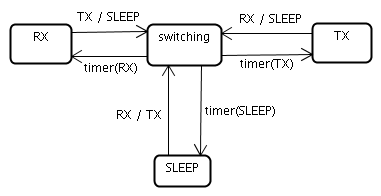
\includegraphics[width=240pt]{req_spec/stateMachineMode.png}
 % stateMachineMode.png: 1179666x1179666 pixel, 0dpi, infxinf cm, bb=
 \caption{State machine for radiostate}
 \label{fig: mode state machine}
\end{figure}


\subsection{send packets}
\label{subSendPackets}

The physical layer has to be able to send packets from the MAC layer to the channel. 
We also want to support the possibility to control
the sending process after it has been started.\reqdefLabel{defsendControl}

Before we can send packets the following things have to be 
assured:
% \linebreak
\begin{itemize}
 \item the radio has to be in TX state\reqdefLabel{defsendPreqMode}
 \item we are not already sending\reqdefLabel{defsendPreqSending}
% \item the channel should be idle (this is no hard requirement)\reqdefLabel{defsendPreqIdle}
\end{itemize}

The above items should be controlled by the MAC layer so the physical layer would only throw an error if they are not set.

The following information has to be attached by the MAC layer to the packet:

\begin{itemize}

 %\item channel\reqdefLabel{defsendCtrlChannel}
 \item channel dimensions (frequency/space)\reqdefLabel{defsendCtrlChannel}
 %\item header bitrate\reqdefLabel{defsendCtrlHeaderBitrate}
 %\item payload bitrate\reqdefLabel{defsendCtrlBitrate}
 \item bitrate (for all dimensions) over time\reqdefLabel{defsendCtrlHeaderBitrate}\reqdefLabel{defsendCtrlBitrate}\\
 \emph{Note: Most cases will be covered by header and payload bitrate.}
 \item TX power for all dimensions over time\reqdefLabel{defsendCtrlTXPower}
 
 \item size of packet\reqdefLabel{defsendCtrlSize}
\end{itemize}


The sending process itself is made up of the following steps:

\begin{enumerate}\reqdefLabel{defpacketFromMac}\reqdefLabel{defsendInfoTXPower}\reqdefLabel{deftxover2}\reqdefLabel{defsendToChannel}
 \item MAC layer gives packet and control info to physical layer
 \item check requirements for sending, throw error if they are not fulfilled
 \item add information needed by the receiving physical layer to packet (see below)
 %\item add signal function (transmission power\footnote{The receiver converts the same signal to receiving power over time.} over time)\footnote{The signal function could be more dimensional. E.g.: receiving power over time and channel.} to packet
 \item add signal to packet
 \item packet is sent to channel by physical layer
 \item schedule transmission over message for MAC layer
\end{enumerate}

The following information is needed by the receiving physical layer:

\begin{itemize}
\item signal
	\begin{itemize}
	\item TX power (for all dimensions) over time
	\item the bitrate (for all dimensions) over time\reqdefLabel{defsendInfoBitrate} 
	\item the channel(dimensions)\reqdefLabel{defsendInfoChannel}
	\item the duration the signal would need to be transmitted\reqdefLabel		{defsendInfoDuration}
	\item the duration of the preamble\reqdefLabel{defsendInfoPreambleDuration}
	
	\end{itemize}
\item position, move direction and speed of the sending host\reqdefLabel{defsendInfoMove}
\item size of packet\reqdefLabel{defsendInfoSize}
\end{itemize}

\subsection{receive packets}
\label{receivePackets}

Because the packets arrive immediately at every receiving node we have to
simulate the receiving process:

\begin{enumerate}\reqdefLabel{defrcvSimDelay}\reqdefLabel{defrcvSimPreamble}\reqdefLabel{defrcvSimDuration}
\item simulate propagation delay (if needed)
\item simulate preamble duration
\item simulate payload duration
\end{enumerate}

We also have to simulate the attenuation of the signal strength\reqdefLabel{defrcvSimAttenuation}. This should be done by filtering the signal with the \textit{analogue models} directly after a message arrives (since we already have it then). The AnalogueModels will add an attenuation matrix to the Signal.\\

%If the preamble is transmitted the packet has to be classified as
\textit{signal} or \textit{noise}\reqdefLabel{defrcvClassify}. The decision is
made by the \textit{Decider}. Therefore the preamble has to be filtered
previously by the analogue models.\reqdefLabel{defrcvFilterPreamble}

The packet has to be classified as \textit{signal} or
\textit{noise}\reqdefLabel{defrcvClassify}. The decision is made by the
\textit{Decider}.\\

If the transmission of a \textit{signal} is over we have to decide if it was
received correctly.\reqdefLabel{defrcvIsCorrect} This is also done by the
\textit{Decider} by evaluating the \textit{signal to noise ratio} short
\textit{SNR}. 
If the signal was received correctly we pass it to the MAC
layer.\reqdefLabel{defrcvPassToMAC} It is also possible to pass the signal to
the MAC layer anyway, marked as biterror/collision.

\subsubsection{the analogue model}
\label{analogueModel}

The \textit{analogue model} simulates the attenuation of the signal strength by
filtering the receiving power function\reqdefLabel{defanalogueFilter}.

There should be models to simulate the following things:

\begin{itemize}
 \item pathloss\reqdefLabel{defanalogueSimPathloss}
 \item shadowing\reqdefLabel{defanalogueSimShadowing}
 \item fading\reqdefLabel{defanalogueSimFading}
\end{itemize}

Further we set the following requirements to the \textit{analogue models}:

\begin{itemize}
 \item physical layer should be able to apply multiple \textit{analogue models}
to a signal\reqdefLabel{defanalogueMulti}
 \item you should be able to set the \textit{analogue models} independent from
physical layer\reqdefLabel{defanalogueIndependent}
 \item you should be able to add your own \textit{analogue
models}\reqdefLabel{defanalogueExtensible}
\end{itemize}

\subsubsection{the Decider}
\label{Decider}

As mentioned already above the \textit{Decider} has to decide the following
things:

\begin{itemize}
\item classify packet as \textit{signal} or
\textit{noise}\reqdefLabel{defrcvClassify2}
\item decide if a packet was received correctly on the basis of the signal and 
interfering noise\reqdefLabel{defrcvIsCorrect2}
\end{itemize}

We set the following requirements to the \textit{Decider}:

\begin{itemize}
 \item you should be able to set the \textit{Decider} independently from
physical layer\reqdefLabel{defdeciderIndependent}
 \item you should be able to add your own
\textit{Decider}\reqdefLabel{defdeciderExtensible}
 \item the \textit{Decider} should be able to return bitwise correctness of the
\textit{signal} (on demand)\reqdefLabel{defdeciderBitwise}
\end{itemize}


\subsection{statistical information}
\label{statistic}

You should be able to get the following statistical information (the physical
layer should not evaluate it but has to provide access to the according
information):

\begin{itemize}
\item packet count\reqdefLabel{defstatPackets}
\item received signal strength\reqdefLabel{defstatRSS}
\item signal to noise ratio\reqdefLabel{defstatSNR}
\item bit error ratio\reqdefLabel{defstatBER}
\item collisions\reqdefLabel{defstatColls}
\end{itemize}

\subsection{parameters}
\label{parameters}

The following parameters of the physical layer should be freely configurable:

\begin{itemize}
	\item simulate propagation delay? (boolean)\reqdefLabel{defconfDelay}
	\item which analogue models should be used\reqdefLabel{defconfAnalogue}
	\item the parameters for the analogue models\reqdefLabel{defconfAnalogueParam}
	\item which Decider should be used\reqdefLabel{defconfDecider}
	\item the parameters for the decider\reqdefLabel{defconfDeciderParam}
	\item thermal noise\reqdefLabel{defconfNoise}
	\item sensitivity\reqdefLabel{defconfSens}
	\item maximum TX power\reqdefLabel{defconfMaxTXPower}
	\item switching times between states (RX, TX, SLEEP)\reqdefLabel{defconfSwitchingTimes}
\end{itemize}




